\documentclass[10pt,a4paper,twocolumn,twoside]{article}
\usepackage[utf8]{inputenc}
\usepackage[catalan]{babel}
\usepackage{multicol}
\usepackage{graphicx}
\usepackage{fancyhdr}
\usepackage{times}
\usepackage{titlesec}
\usepackage{url}
\usepackage{multirow}
\usepackage{lettrine}
\usepackage[top=2cm, bottom=1.5cm, left=2cm, right=2cm]{geometry}
\usepackage[figurename=Fig.,tablename=TAULA]{caption}
\captionsetup[table]{textfont=sc}

\author{\LARGE\sffamily Miquel Freixes Faya}
\title{\Huge{\sffamily Anàlisis de la relació entre les emisions de Co2 i l'augment de la temperatura, mitjançant tècniques i tecnologies de Big Data. 1r Informe de Seguiment}}
\date{}

\newcommand\blfootnote[1]{%
  \begingroup
  \renewcommand\thefootnote{}\footnote{#1}%
  \addtocounter{footnote}{-1}%
  \endgroup
}

%
%\large\bfseries\sffamily
\titleformat{\section}
{\large\sffamily\scshape\bfseries}
{\textbf{\thesection}}{1em}{}

\begin{document}

\fancyhead[LO]{\scriptsize MIQUEL FREIXES FAYA: TÍTOL DEL TREBALL}
\fancyhead[RO]{\thepage}
\fancyhead[LE]{\thepage}
\fancyhead[RE]{\scriptsize EE/UAB TFG INFORMÀTICA: TÍTOL (ABREUJAT SI ÉS MOLT LLARG)}

\fancyfoot[CO,CE]{}

\fancypagestyle{primerapagina}
{
   \fancyhf{}
   \fancyhead[L]{\scriptsize TFG EN ENGINYERIA INFORMÀTICA, ESCOLA D'ENGINYERIA (EE), UNIVERSITAT AUTÒNOMA DE BARCELONA (UAB)}
   \fancyfoot[C]{\scriptsize ``Febrer'' de 2019, Escola d'Enginyeria (UAB)}
}

%\lhead{\thepage}
%\chead{}
%\rhead{\tiny EE/UAB TFG INFORMÀTICA: TÍTOL (ABREUJAT SI ÉS MOLT LLARG)}
%\lhead{ EE/UAB \thepage}
%\lfoot{}
%\cfoot{\tiny{February 2015, Escola d'Enginyeria (UAB)}}
%\rfoot{}
\renewcommand{\headrulewidth}{0pt}
\renewcommand{\footrulewidth}{0pt}
\pagestyle{fancy}

%\thispagestyle{myheadings}
\twocolumn[\begin{@twocolumnfalse}

%\vspace*{-1cm}{\scriptsize TFG EN ENGINYERIA INFORMÀTICA, ESCOLA D'ENGINYERIA (EE), UNIVERSITAT AUTÒNOMA DE BARCELONA (UAB)}

\maketitle

\thispagestyle{primerapagina}
%\twocolumn[\begin{@twocolumnfalse}
%\maketitle
%\begin{abstract}
\begin{center}

{\vrule depth 0pt height 0.5pt width 4cm\hspace{7.5pt}%
\raisebox{-3.5pt}{\fontfamily{pzd}\fontencoding{U}\fontseries{m}\fontshape{n}\fontsize{11}{12}\selectfont\char70}%
\hspace{7.5pt}\vrule depth 0pt height 0.5pt width 4cm\relax}

\end{center}

\bigskip
%\end{abstract}
\end{@twocolumnfalse}]

\blfootnote{$\bullet$ E-mail de contacte: m.freixes.faya@gmail.com}
\blfootnote{$\bullet$ Menció realitzada: Tecnologies de la Informació}
\blfootnote{$\bullet$ Treball tutoritzat per: Jordi Casas Roma (departament)}
\blfootnote{$\bullet$ Curs 2018/19}

\section{Evolució dels Objectius}
\lettrine[lines=3]{L}{'objectiu} principal d'aquest treball segueix sent el mateix que l'esmentat anteriorment, analitzar el canvi de temperatura al llarg dels anys. El que sí que ha canviat són els paràmetres amb els quals es compararà la temperatura. En lloc de fer-ho amb la petjada ecològica i les emissions de Diòxid de Carboni (CO$_2$), com s'havia plantejat en un inici, es farà amb les emissions de tres gasos hivernacle. També s'ha decidit reduir l'àrea d'on s'agafaran les dades, en lloc de fer-ho de tota la Terra es focalitzarà en el continent d'Europa, concretament en els països dins de la Unió Europea.

El primer canvi s'ha decidit després d'analitzar els \textit{DataSets} amb més detall i veure que tenia més sentit comparar els canvis de temperatura amb les principals causes que podien provocar-los. Per tant s'ha decidit agafar només les dades sobre les emissions de CO$_2$, les de Metà (CH$_4$) i les d'òxid de nitrogen (N$_2$O). La comparació inicial també complicava bastant el treball,a causa de la complexitat de les fórmules i conceptes involucrats en el \textit{DataSet} de la petjada ecològica. Com el treball està enfocat en el tractament de les dades i ala seva anàlisi, s'ha trobat més coherent agafar conceptes menys complicats per poder dedicar més temps en el seu processament.

El segon té una justificació semblant, agafant els països dins de la Unió Europea s'obtenen unes 22000 files d'informació i agafar més països hauria produït un augment del temps d'entrenament de l'algorisme, causant una extensió de la planificació. Com s'ha esmentat anteriorment, com l'objectiu és dins de l'àmbit informàtic, hi ha suficient amb un gruix de dades de més de 20000 files per assolir-lo, per tant es descartaran la resta de països. A més, a Europa hi ha una combinació de països curiosa, ja que hi ha alguns que han reduït dràsticament les emissions mentre d'altres que les han anat pujant o mantingut al llarg dels anys.

\section{ Evolució de la Planificació}
La planificació s'està seguint tal com es va acordar a l'informe inicial. Hi ha un retard d'aproximadament una setmana, a causa del fet que no es va considerar la redacció dels informes. Per arreglar-ho s'ha sumat una setmana més després de cada fase del projecte per editar l'informe.

\section{Evolució de la Metodologia}
A la figura 1 es pot veure com s'hi ha aplicat el mètode Kanban en aquesta primera tasca. S'ha decidit seguir la metodologia per cada fase i no de tot el projecte a la vegada. Així, es pot mantenir un seguiment més concís de les tasques de cada una de les fases i poder prioritzar-les millor. Per fer-ho simple, s'han creat tres columnes de tasques: Les que s'han de fer, les que s'estan fent i les que estan fetes. Així es pot veure tota la feina feta, la que s'està fent i la que queda per fer podent planejar-se segons avanci el projecte. També es pot veure el repositori on de moment només hi ha penjat els arxius dels informes, fonts d'informació i els \textit{DataSets} [1]. Això és degut al fet que tot el codi s'ha escrit per la interfície en línia de DataBricks, el qual ja té un repositori incorporat, i s'ha trobat innecessari replicar els commits que es feien al repositori local.
\section{Preprocessament de dades}
Per començar s'han importat els dos \textit{DataSets} des del seu csv corresponent:
%taula2
\begin{table}[ht]
\caption{Taula de temperatures}
\begin{center}
\begin{tabular}{c c c c} % centered columns (4 columns)
\hline\hline %inserts double horizontal lines
dt & Temp & Average & Country \\
\hline
01-01-1750 & 1.12 & 2.245 & Germany \\
01-02-1750 & 2.234 & 1.3 & Germany \\
\hline
\end{tabular}
\end{center}
\end{table}
\begin{itemize}
\item El primer està format de quatre columnes, tal com es mostra a la taula 1 hi ha una amb la data, en format String amb dies mesos i anys. El segon valor és la temperatura mesurada amb un marge d'error del 95\%, serà el valor que es donarà per vàlid al llarg del treball. El tercer és el marge d'error que pot tenir la temperatura de la segona columna i l'última el nom del país al qual s'està mesurant les temperatures. Aquest \textit{DataSet} està extret de Kaggle, però és una recopilació d'investigacions fetes per Berkeley Earth [2]. És una empresa sense ànim de lucre destinada a revisar i documentar l'increment de temperatura al llarg dels anys [3]. Aquest \textit{DataSet} és una compressió de dades extretes de més d'1,6 bilions de registres entre els anys 1750 i el 2013 de tot el món per cada mes de l'any.

%taula2
\begin{table}[ht]
\caption{Taula de gasos}
\begin{center}
\begin{tabular}{c c c c} % centered columns (4 columns)
\hline\hline %inserts double horizontal lines
Country & Year & Value & Type \\
\hline
Germany & 1990 & 432012.435 & Co2\_lulucf \\
Germany & 1990 & 474532.8236 & CH4\_lulucf \\
Germany & 1990 & 29645.74 & N2O\_lulucf \\
\hline
\end{tabular}
\end{center}
\end{table}
\item El segon està compost pel mateix nombre de columnes. Com es pot veure a la taula 2, és bastant semblant a l'anterior. La primera és el nom del país on s'està mesurant, la segona és l'any on s'ha mesurat, aquest cop en format d'enter. En la tercera tenim el valor de la mitjana de Kilotones de gas produït per capita en el país, i en l'última tenim el tipus de gas que s'ha mesurat i quins paràmetres s'han utilitzat per fer-ho. En aquest \textit{DataSet} s'han extret les dades de les emissions de cada país, dels diferents gasos hivernacle des de l'any 1990 al 2013 [4]. La majoria de mesures estan extretes sense considerar les activitats d'ús de la terra o d'intercanvi de recursos amb la terra, anomenades en anglès com a LULUCF (\textit{Land Use, Land-Use Change and Forestry}). Bàsicament aquestes activitats comprenen alguns sectors de l'agricultura i/o obtenció de matèries primeres [5]. Aquestes activitats representen un 7\% del total d'emissions, per tant s'analitzarà en el treball el 93\% restant que representa tots els altres sectors com el de la indústria, el turisme, el consum particular, entre d'altres [6].
 
\end{itemize}

Un cop entesos els \textit{DataSets} es pot començar amb el seu tractament. Per fer-lo s'ha utilitzat l'eina en línia de Databricks, optimitzada per treballar amb Spark, a més de permetre treballar amb Pandas i d'altres frameworks o llibreries de processament de dades. Aquesta eina té una versió de pagament i una gratuïta, en aquest treball s'ha escollit la gratuïta que proporciona un clúster amb un màxim de 6Gb de RAM [7]. S'ha preferit utilitzar aquesta opció, ja que ha evitat tot el procés de muntar un sistema en una màquina per treballar amb Spark, permetent dedicar més temps al processament de les dades. En aquesta eina s'ha utilitzat el \textit{framework} de pySpark, i diverses llibreries com Pandas, Numpy i SciPy.

Per una banda tenim Pandas, una llibreria de codi obert amb llicència de \textit{Berkeley Distributed Systems} optimitzada per al processament de grans volums de dades. Aquesta llibreria proporciona estructures de dades que són flexibles i ràpides que permet treballar amb elles d'una forma fàcil. El seu element bàsic és el \textit{DataFrame}, que es pot representar com una taula amb files i columnes. Aquest element és molt més fàcil i eficient que un diccionari o una llista gràcies al fet que no cal implementar estructures de bucles molt complicades per anar iterant sobre els seus valors [8].

Per l'altra banda tenim Spark, un entorn creat per obtenir un processament i una anàlisi de grans quantitats de dades en entorns distribuïts, obtenint un alt rendiment i una gran velocitat. Això ho aconsegueix a partir de distribuir les dades pel clúster i treballant en memòria, no en disc. En programar el treball en Python s'ha utilitzat el framework pySpark, bàsicament ofereix totes les eines de Spark pel llenguatge. L'element més bàsic i important en Spark és el \textit{resilient distributed dataset} o RDD, és la base de la seva estructura de paral·lelització. El RDD és un objecte abstracte que representa un conjunt de dades, que estan distribuïdes pel clúster. Aquests objectes són immutables i poden emmagatzemar-se en memòria [9]. A banda dels RDD, un altre element important és el \textit{DataFrame}. Aquest element és un concepte pràcticament idèntic al \textit{DataFrame} utilitzat per Pandas. Utilitzant DataBricks els \textit{DataFrames} de Spark es poden visualitzar de moltes maneres diferents gràcies a l'interfície que ofereix l'eina.

Amb aquestes dues opcions sobre la taula, s'ha preferit començar utilitzant Spark gràcies al fet que l'eina de DataBricks estava optimitzada per ella. Primer s'ha importat els dos \textit{DataSets} i se'ls ha transformat a \textit{DataFrames}. Un cop fet iniciat el procediment de canviar les dades, tant el nombre de dades com el format, s'ha començat a trobar alguns problemes ja que no s'acabava de trobar la manera de fer alguns canvis necessaris per treure el format correcte. Per exemple, era difícil iterar cada fila canviant valors específics en cada una d'elles. Per poder fer aquests processos s'ha decidit passar els \textit{DataFrames} a la llibreria Pandas. Aquesta decisió ha anat condicionada pel gran volum d'informació que hi ha a Internet sobre com fer el tractament de dades en Pandas i també per la facilitat que proporciona la llibreria amb algunes llibreries científiques com Numpy i SciPy.

Un cop passats a \textit{DataFrames}de Pandas s'han modificat i adaptat cada un per després unir-los en un de sol:
\begin{itemize}
\item Amb el de les temperatures, s'ha començat descartant tots els anys que no té el \textit{DataSet} de les emissions, a causa del fet que l'algorisme de \textit{Machine Learning} ha d'agafar el mateix període de temps per poder comparar els valors. Un cop descartats s'ha quedat el període de 1990 al 2012, amb dotze mesures mensuals per cada any. A partir d'aquí, s'ha descartat tots els països que no estiguin dins de la Unió Europea i s'ha canviat el format de les dates, passant-les de String a enter i eliminant els dies.
\item El de les emissions ha estat una mica més complicat de modificar. Primer s'ha hagut de filtrar els gasos i països desitjats, per descartar totes les dades innecessàries. Després, ha aparegut el principal problema, en aquest \textit{DataFrame} les mesures es fan per any, no per mes com en el de les temperatures. Per solucionar-ho primer s'ha plantejat el fet de canviar les temperatures a mesures anuals, fent la mitjana de les mensuals, però el nombre de files restants no arribava a les mínimes per treure resultats bons amb els algorismes de \textit{Machine Learning}. Com l'única solució restant era transformar una mesura per any a una per més, ha calgut fer una interpolació de les dades.

Una interpolació és el mètode matemàtic que permet construir un conjunt de punts a partir d'uns de coneguts. Existeixen diversos tipus d'interpolació, d'entre les quals s'ha considerat aplicar en aquest treball la lineal, la polinòmica i la de traçadors. La primera s'ha descartat a causa de la poca precisió que aporta en la creació de nous punts. La segona s'ha considerat com una opció viable, però té un hàndicap molt gran amb polinomis de graus elevats anomenat el Síndrome de Runge, en el cas d'aquest treball és de grau 12. Aquest fenomen provoca una gran desviació de les dades als extrems i al centre de la interpolació, afectant greument a la precisió de les dades [10]. Per evitar aquest fenomen s'ha aplicat el tercer mètode d'interpolació. Aquest consisteix a dividir els punts coneguts en polinomis de grau tres, aquests polinomis es poden interpolar amb la interpolació polinòmica, evitant el fenomen de Runge gràcies al seu grau baix. Un cop interpolats, es van encadenant un darrere l'altre aconseguint la gràfica completa amb tots els punts desitjats. Amb aquest mètode s'aconsegueix evitar les desviacions a més d'aconseguir una bona precisió en els punts creats [11]. Havent escollit el mètode d'interpolació, s'ha buscat la millor manera de programar-ho en Python i s'ha utilitzat un mètode de la llibreria SciPy [12] on només cal enviar-li els punts coneguts i el nombre de punts que es vol aconseguir per cada interpolació. Per crear els punts s'ha utilitzat una funció d'una altra llibreria, Numpy, la qual ha transformat els anys i les quantitats en les coordenades x i y d'un punt.
\end{itemize}
Un cop editats els dos \textit{DataFrames} per separat s'han unit en un de sol i s'ha passat a un \textit{DataFrame} de Spark per poder visualitzar-lo millor. Gràcies a les eines que ofereix Databricks per fer múltiples gràfiques a partir de les dades en Spark es pot observar bé si hi ha hagut errors en aquest procés, o si hi ha algun tipus d'inconsistència en les dades. Un cop revisades les dades d'aquest últim \textit{DataFrame} s'ha exportat a un fitxer csv que serà el que utilitzarà l'algorisme de \textit{Machine Learning}.
\begin{thebibliography}{11}
\bibitem{1}
Miquel Freixes, ``Treball de Fi de Grau de Miquel Freixes". \textit{GitHub}. [En línia]. Disponible a: \url{ https://github.com/miky96/TFG}. [Accedit Novembre 10, 2018].
\bibitem{2}
``Climate Change: Earth Surface Temperature Data”, \textit{Berkeley Earth}. [En línia]. Disponible a: \url{ https://www.kaggle.com/unitednations/international-greenhouse-gas-emissions}. [Accedit Novembre 9, 2018].
\bibitem{3}
``About Berkjeley Earth", \textit{Berkeley Earth}. [En línia]. Disponible a: \url{http://berkeleyearth.org/about/}. [Accedit Novembre 9, 2018].
\bibitem{4}
 ``International Greenhouse Gas Emissions”, \textit{United Nations}. [En línia]. Disponible a: \url{ https://www.kaggle.com/unitednations/international-greenhouse-gas-emissions}. [Accedit Novembre 9, 2018].
\bibitem{5}
 ``Land Use, Land-Use Change and Forestry (LULUCF)", \textit{United Nations}. [En línia]. Disponible a: \url{ https://unfccc.int/topics/land-use/workstreams/land-use--land-use-change-lulucf}. [Accedit Novembre 7, 2018].
\bibitem{6}
Federica Pozzi, ``Lmportancia del recuento del UTCUTS (LULUCF) para el éxito del Acuerdo de París". \textit{Carbon Market Watch}. [En línia]. Disponible a: \url{https://carbonmarketwatch.org/es/2017/07/18/29671/}. [Accedit Novembre 7, 2018].
\bibitem{7}
``Databricks Unified Analytics", \textit{DataBricks}. [En línia]. Disponible a: \url{https://databricks.com/}. [Accedit Novembre 6, 2018].
\bibitem{8}
 ``Python Data Analysis Library", \textit{Pandas}. [En línia]. Disponible a: \url{https://pandas.pydata.org/}. [Accedit Novembre 7, 2018].
\bibitem{9}
F.Julbe, \textit{Anàlisi de dades massives: Tècniques fonamentals}. Barcelona, UOC. Pàgines: 30-32.
\bibitem{10}
B.Fornberg, J.Zuev. \textit{The Runge phenomenon and spatially variable shape parameters in RBF interpolation}. University Of Colorado.
\bibitem{11}
 ``Interpolation", \textit{Wikipedia}. [En línia]. Disponible a: \url{https://en.wikipedia.org/wiki/Interpolation#Spline_interpolation}. [Accedit Novembre 10, 2018].
\bibitem{12}
 ``scipy.interpolate.InterpolatedUnivariateSpline", \textit{SciPy}. [En línia]. Disponible a: \url{https://docs.scipy.org/doc/scipy/reference/generated/scipy.interpolate.InterpolatedUnivariateSpline.html}. [Accedit Novembre 10, 2018].
\end{thebibliography}
\clearpage
\section{Annex}

\begin{figure}[!h]
\centering
	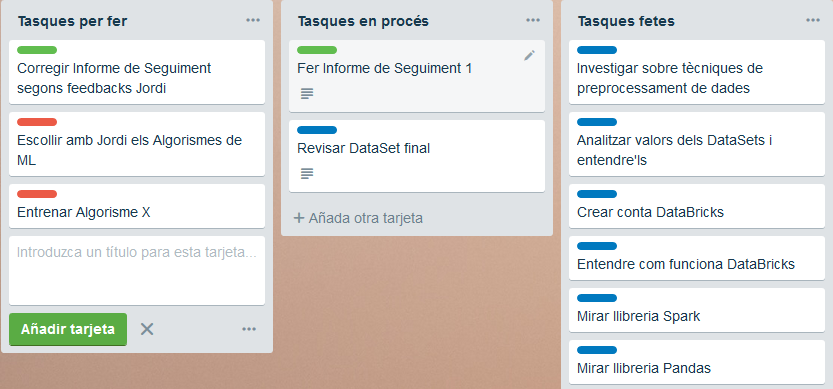
\includegraphics[width=1\textwidth]{img/kanban}

	\caption{Panell Kanban}
	\label{fig-Kanban}
\end{figure}


\end{document}

